%%%%%%%%%%%%%%%%%%%%%%%%%%%%%%%%%%%%%%%%%%%%%%%%%%%%%%%%%%%%%%%%%%%%%%%%%
%%%  LaTeX format of the thesis of the Gyeonggi Science High School   %%%
%%%  Last edition (2015.11.21) by Chinook Mok                         %%%
%%%%%%%%%%%%%%%%%%%%%%%%%%%%%%%%%%%%%%%%%%%%%%%%%%%%%%%%%%%%%%%%%%%%%%%%%

\documentclass[twoside,11pt]{gshs_thesis}
\RequirePackage[nonfrench]{kotex}
\usepackage[percent]{overpic}
\usepackage{verbatim}
\usepackage{tikz}
\usepackage{amssymb}
\graphicspath{{./images/}}
% -----------------------------------------------------------------------
%                   이 부분은 수정하지 마시오.
% -----------------------------------------------------------------------
\titleheader{졸업논문청구논문}
\school{과학영재학교 경기과학고등학교}
\approval{위 논문은 과학영재학교 경기과학고등학교 졸업논문으로\\
졸업논문심사위원회에서 심사 통과하였음.}
\chairperson{심사위원장}
\examiner{심사위원}
\apprvsign{(인)}
\korabstract{초 록}
\koracknowledgement{감사의 글}
\korresearches{연 구 활 동}

%: ----------------------------------------------------------------------
%:                  논문 제목과 저자 이름을 입력하시오
% ----------------------------------------------------------------------
\title{소형 천체망원경의 아크릴 바흐티노프마스크 원격 제어를 위한 덮개 개발} %한글 제목
\engtitle{Development of a Cover for the Control of Acrylic Bahtinov Mask for a Small Astrophysical Telescope} %영문 제목
\korname{곽 지 성} %저자 이름을 한글로 입력하시오 (글자 사이 띄어쓰기)
\engname{Gwak, Ji-Seong} %저자 이름을 영어로 입력하시오 (family name, personal name)
\chnname{郭 志 誠} %저자 이름을 한자로 입력하시오 (글자 사이 띄어쓰기)
\studid{18008} %학번을 입력하시오

%------------------------------------------------------------------------
%                  심사위원과 논문 승인 날짜를 입력하시오
%------------------------------------------------------------------------
\advisor{Mok, Chinook}  %지도교사 영문 이름 (family name, personal name)
\judgeone{박 교 수} %심사위원장
\judgetwo{김 대 감}   %심사위원1
\judgethree{박 기 현} %심사위원2(지도교사)
\degreeyear{2021}   %졸업 년도
\degreedate{2019. 6. 18} %논문 승인 날짜 양식1
\degreedatekor{2019년 6월 18일} %논문 승인 날짜 양식2

%------------------------------------------------------------------------
%                  논문제출 전 체크리스트를 확인하시오
%------------------------------------------------------------------------
\checklisttitle{[논문제출 전 체크리스트]} %수정하지 마시오
\checklistI{1. 이 논문은 내가 직접 연구하고 작성한 것이다.} %수정하지 마시오
% 이 항목이 사실이라면 다음 줄 앞에 "%"기호 삽입, 다다음 줄 앞의 "%"기호 제거하시오
\checklistmarkI{$\square$}
%\checklistmarkI{$\text{\rlap{$\checkmark$}}\square$}
\checklistII{2. 인용한 모든 자료(책, 논문, 인터넷자료 등)의 인용표시를 바르게 하였다.} %수정하지 마시오
% 이 항목이 사실이라면 다음 줄 앞에 "%"기호 삽입, 다다음 줄 앞의 "%"기호 제거하시오
\checklistmarkII{$\square$}
%\checklistmarkII{$\text{\rlap{$\checkmark$}}\square$}
\checklistIII{3. 인용한 자료의 표현이나 내용을 왜곡하지 않았다.} %수정하지마시오
% 이 항목이 사실이라면 다음 줄 앞에 "%"기호 삽입, 다다음 줄 앞의 "%"기호 제거하시오
\checklistmarkIII{$\square$}
%\checklistmarkIII{$\text{\rlap{$\checkmark$}}\square$}
\checklistIV{4. 정확한 출처제시 없이 다른 사람의 글이나 아이디어를 가져오지 않았다.} %수정하지 마시오
% 이 항목이 사실이라면 다음 줄 앞에 "%"기호 삽입, 다다음 줄 앞의 "%"기호 제거하시오
\checklistmarkIV{$\square$}
%\checklistmarkIV{$\text{\rlap{$\checkmark$}}\square$}
\checklistV{5. 논문 작성 중 도표나 데이터를 조작(위조 혹은 변조)하지 않았다.} %수정하지 마시오
% 이 항목이 사실이라면 다음 줄 앞에 "%"기호 삽입, 다다음 줄 앞의 "%"기호 제거하시오
\checklistmarkV{$\square$}
%\checklistmarkV{$\text{\rlap{$\checkmark$}}\square$}
\checklistVI{6. 다른 친구와 같은 내용의 논문을 제출하지 않았다.} %수정하지 마시오
% 이 항목이 사실이라면 다음 줄 앞에 "%"기호 삽입, 다다음 줄 앞의 "%"기호 제거하시오
\checklistmarkVI{$\square$}
%\checklistmarkVI{$\text{\rlap{$\checkmark$}}\square$}


\begin{document}
\renewcommand\baselinestretch{1.4} % line spacing in the paragraph
\baselineskip=22pt plus1pt         % line spacing in the paragraph

\maketitle  % command to print the title page with above variables
\setcounter{page}{1}
%---------------------------------------------------------------------
%                  영문 초록을 입력하시오
%---------------------------------------------------------------------
\begin{abstracts}     %this creates the heading for the abstract page
\noindent{
Put your abstract here. It is completely consistent with 한글초록.
}
\end{abstracts}

%---------------------------------------------------------------------
%                  국문 초록을 입력하시오
%---------------------------------------------------------------------
\begin{abstractskor}        %this creates the heading for the abstract page
\noindent{
본 연구에서 소형 천체망원경의 아크릴 바흐티노프마스크 원격제어가 가능한 제어시스템인 GS-system를 개발하였다. GS-system은 기존에 개발한 모터포커서를 사용하되, 바흐티노프마스크의 원격 제어 및 다른 여러 기능을 탑재하여 사용의 편의성을 증대시켰으며, 이를 사용하여 특정 소형 천체망원경에 사용할 수 있는 바흐티노프마스크 제어용 덮개를 제어할 수 있도록 하였다. GS-system을 통해 소형 천체망원경에 사용되는 바흐티노프마스크의 제어를 편리하게 할 수 있으며, 천체 관측에 필요한 기능들 또한 ASCOM 드라이버와 호환되는 소프트웨어들을 통한 GUI (graphical user interface)를 활용해 편리하게 사용할 수 있도록 하였다. 
}
\end{abstractskor}

	\begin{comment}
초록(요약문)은 가장 마지막에 작성한다. 연구한 내용, 즉 본론부터 요약한다. 서론 요약은 하지 않는다. 대개 첫 문장은 연구 주제 (+방법을 핵심적으로 나타낼 수 있는 문구: 실험적으로, 이론적으로, 시뮬레이션을 통해)를 쓴다. 다음으로 연구 방법을 요약한다. 선행 연구들과 구별되는 특징을 중심으로 쓴다. 뚜렷한 특징이 없다면 연구방법은 안써도 상관없다. 다음으로 연구 결과를 쓴다. 연구 결과는 추론을 담지 않고, 객관적으로 서술한다. 마지막으로 결론을 쓴다. 이 연구를 통해 주장하고자 하는 바를 간략히 쓴다. 요약문 전체에서 연구 결과와 결론이 차지하는 비율이 절반이 넘도록 한다. 읽는 이가 요약문으로부터 얻으려는 정보는 연구 결과와 결론이기 때문이다. 연구 결과만 레포트하는 논문인 경우, 결론을 쓰지 않는 경우도 있다.
	\end{comment}
%----------------------------------------------
%   Table of Contents (자동 작성됨)
%----------------------------------------------
\setcounter{secnumdepth}{3} % organisational level that receives a numbers
\setcounter{tocdepth}{3}    % print table of contents for level 3
\tableofcontents


%----------------------------------------------
%     List of Figures/Tables (자동 작성됨)
%----------------------------------------------
\cleardoublepage
\clearpage
\listoffigures	% 그림 목록과 캡션을 출력한다. 만약 논문에 그림이 없다면 이 줄의 맨 앞에 %기호를 넣어서 코멘트 처리한다.

\cleardoublepage
\clearpage
\listoftables  % 표 목록과 캡션을 출력한다. 만약 논문에 표가 없다면 이 줄의 맨 앞에 %기호를 넣어서 코멘트 처리한다.


%%%%%%%%%%%%%%%%%%%%%%%%%%%%%%%%%%%%%%%%%%%%%%%%%%%%%%%%%%%
%%%% Main Document %%%%%%%%%%%%%%%%%%%%%%%%%%%%%%%%%%%%%%%%
%%%%%%%%%%%%%%%%%%%%%%%%%%%%%%%%%%%%%%%%%%%%%%%%%%%%%%%%%%%
\cleardoublepage
\clearpage
\renewcommand{\thepage}{\arabic{page}}
\setcounter{page}{1}


%-----------------------------------------------------
%  Introduction
%-----------------------------------------------------

\section{서론}
\subsection{연구의 필요성}

천체 관측은 천체 망원경이 대중화됨에 따라 여러 사람들이 시도하는 경우가 많아졌다. 하지만 천체관측을 할 시에는 여러 가지 변수가 존재하여, 천체관측을 어렵게 하는 경우가 있다. 천체 관측을 하는 데 중요한 요소 중 하나는 초점을 정확하게 맞추는 것이다. 초점이 얼마나 정확하게 맞았는 지에 따라서 천체관측한 사진의 상이 얼마나 정확하게 나왔는지가 달라질 뿐만이 아니라 장시간 노출을 하여 사진을 촬영해야 하는 밤에 경우 초점이 맞지 않으면 그 차이가 더욱 두드러지게 나타나게 된다. 최근에는 이러한 문제를 해결하기 위해 컴퓨터를 이용하여 정확한 제어를 통해 짧은 시간안에 효율적인 관측을 진행하고자 노력하고 있다.

천체망원경의 초점을 맞추는 대표적인 방법들 중 하나는 천체망원경의 모터포커서를 활용하여 FWHM(Full Width Half Maximum), UFD(Half Flux Diameter)와 같은 값들을 활용한 V-curve를 그려 초점을 찾는 방법을 주로 활용한다. 이 방법을 활용할 경우 어떤 상황에서도 꽤 정확한 결과를 얻을 수 있지만, 이는 별의 flux 정규분포로 퍼져있어야 정확한 결과를 얻을 수 있다. 만약 퍼져있는 정도가 부정확하면 이 결과를 신뢰성이 낮아지게 되며, 천체 관측시의 온도 및 주변 대기의 상태(seeing)에 많은 영향을 받게 된다.

이런 단점들을 개선하기 위해 마스크를 활용하는 방법이 주목받고 있다. 마스크는 크게 하트만 마스크와 바흐티노프 마스크의 두 가지로 나눌 수 있으며, 마스크를 사용하는 방법은 위에서 설명한 방법에 비해 관측시에 필요한 시간을 획기적으로 줄일 수 있다는 장점이 있다. 
본교 보조 관측실은 자동으로 개폐되는 슬라이딩 루프(sliding roof)가 있어, 이곳에 천체망원경을 고정하여 설치해 놓고 관측을 진행하고 있다. 때문에 네트워크만 연결이 되면 언제 어디서든 망원경을 조종할 수 있다는 장점을 가지고 있지만, 아직까지 완전 자동화된 천체관측은 불가능하다.
(마지막 문단 정리하고 싶은데 아예 뺄까 생각중이에요)

\subsection{연구 목적}

바흐티노프마스크의 효율적인 제어를 위하여 소형 천체망원경에 사용할 수 있는 덮개를 제작하여 실제 관측에 사용하는 것을 목적으로 한다. 

제작한 모터 포커서 컨트롤러는 GS-touch로 명명하였다. GS-touch는 스테핑 모터를 구동할 수 있고 컴퓨터로 제어할 수 있도록 설계하였으며, 전용 ASCOM (Astronomy Common Object Model) dirver를 개발하여 ASCOM을 지원하는 천문 소프트웨어를 이용하여 쉽게 사용할 수 있도록 하였다.
본 연구의 또 다른 목적은 관심이 있는 사람들이 직접 부품을 구입하여 제작할 수 있도록 제작과정과 노하우를 공개하여 아이디어 나눔을 실천하는 것도 포함된다.


이를 위해 해결해야 할 주요 문제는 다음과 같다.

\begin{itemize}
\item{덮개는 바흐티노프 마스크를 정확하게 제어할 수 있는가?}\\[-34pt]
\item{바흐티노프 마스크를 이용하여 초점을 정확하게 맞출 수 있는가?}\\[-34pt]
\item{향상된 모터포커서를 이용하여 이들을 제어할 수 있는가?}
\end{itemize}

 	
%-----------------------------------------------------
% Next Section (e.g. Experiment, Linear theory, etc...)
%-----------------------------------------------------
\newpage
\section{이론적 배경}


\subsection{천체 관측 시스템}

\subsection{바흐티노프 마스크}

 바흐티노프 마스크(Bahtinov mask)는 러시아의 아마추어 천문학자인 바흐티노프가 고안한 마스크 중 하나로, 기존에 사용하던 하트만 마스크(Hartmann mask)의 여러 단점을 보완하였기 때문에 이후 주류가 된 마스크의 종류이다. 두 마스크 모두 빛의 회절 현상을 이용한다는 공통점이 있지만, 천체관측에서는 바흐티노프 마스크가 더 포괄적으로 사용된다. 
 
 빛의 회절은 직진하던 빛이 좁은 틈, 슬릿이나 장애물을 통과할 때 물체의 뒤편까지 빛이 나가는 현상으로, 슬릿의 폭이 좁을수록 회절이 잘 일어난다. 바흐티노프 마스크는 Fig. \ref{bahtinov}와 같이 방향이 어긋나있는 세 줄의 회절 슬릿들이 일렬로 나있는 모양을 가지고 있다. 때문에 평행 광선인 별에서 오는 빛이 슬릿을 통과하면 빛은 슬릿에 의해 회절하게 된다. 이 때 빛은 좁은 방향으로 많이 회절하기 때문에 슬릿을 통과한 빛은 통과한 슬릿에 수평한 방향의 선 모양 상을 만들게 된다. 초점이 올바르지 않은 경우에는 평행광이 한점에 모이지 않기 때문에 세 개의 선이 한 점에서 만나지 않지만, 초점이 정확하게 맞추어진 경우에는 상들이 한 점에서 모이기 때문에 세 개의 선이 한 점에서 만나게 된다.
 
 \begin{figure}[h]
 	\begin{center}
 		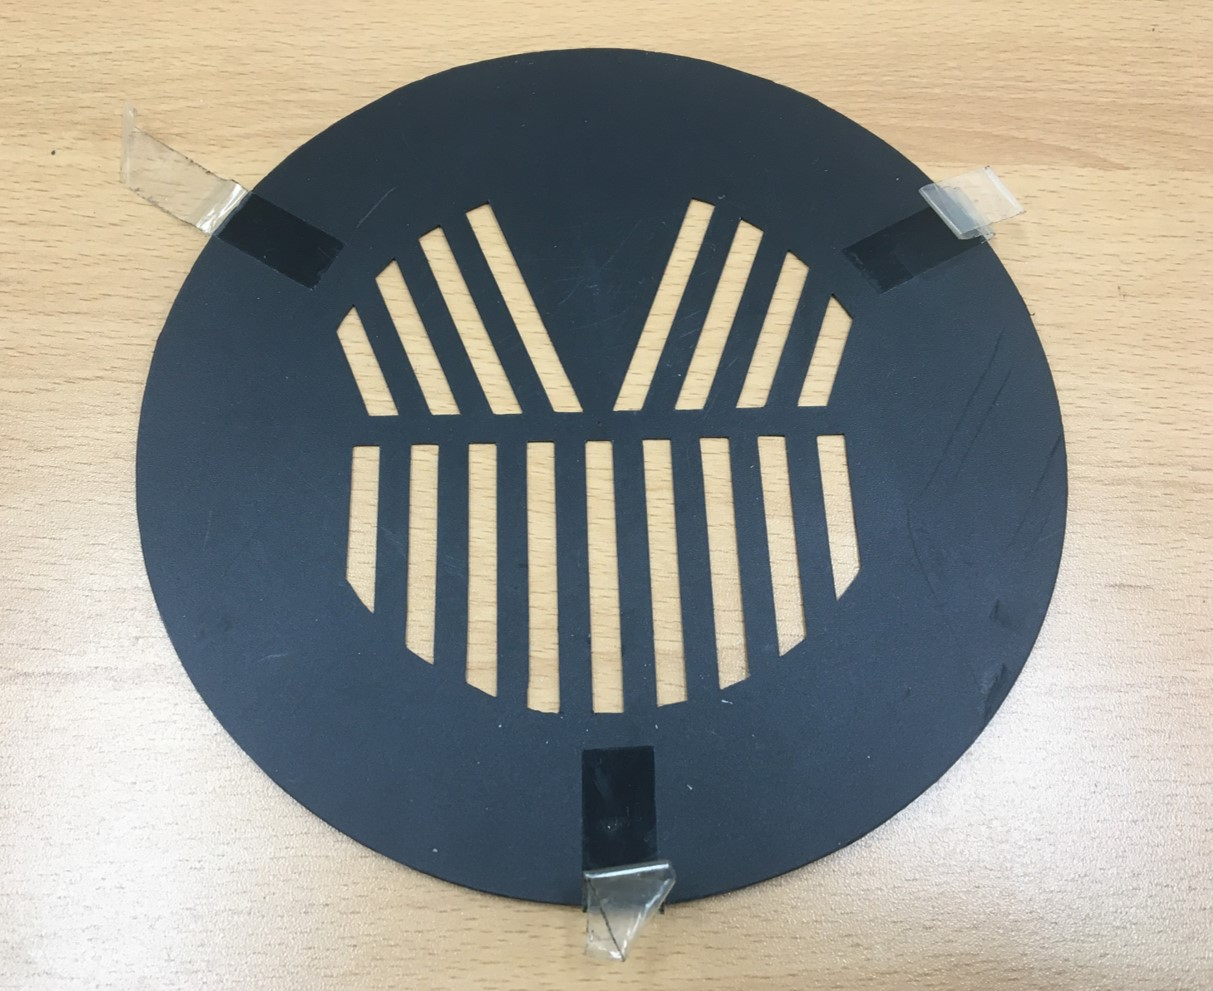
\includegraphics[width = 8cm]{bahtinov1}
 	\end{center}
 	\caption{실제로 천체관측에서 사용되는 바흐티노프 마스크}
 	\label{bahtinow}
 \end{figure}
 
 바흐티노프 마스크는 빛의 회절을 이용하여 초점이 맞았는지 안맞았는지를 쉽고 빠르게 알 수 있기 때문에 시간이 중요한 천체망원경의 초점을 맞추는 데 안성맞춤이다. 회절 슬릿을 이용하기 때문에 아주 밝은 별로만 초점 검출을 할 수 있다는 단점을 가지고 있지만 밤에 천체관측을 하기 위해서는 바흐티노프마스크가 좋은 선택이라고 할 수 있다.
(보완해야합니다)


\subsection{기존 모터포터서 분석 (기존에 존재하는 모터포커서 시스템)}


 이전에 개발된 모터포커서인 GS-touch는 초점을 맞추기 위한 포커서이기 때문에 이를 위한 기능들이 주를 이루었다. 때문에 이를 보완하여 덮개를 제어할 수 있도록 추가로 개발할 필요가 있었다.
 
 \bigskip
 \begin{figure}[h]
 	\begin{center}
 		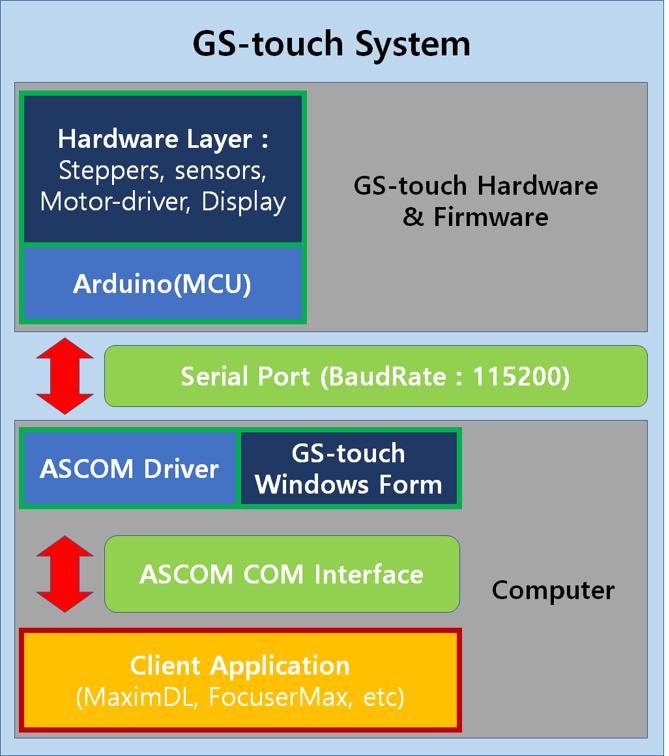
\includegraphics[width = 9.7cm]{GStouch}
 	\end{center}
 	\caption{GS-touch의 주요 기능}
 	\label{GStocuh}
 \end{figure}
  Fig. \ref{GStocuh}는 기존에 사용하는 GS-touch의 주요 기능들을 정리한 표이며, GS-touch는 전체적으로 두 가지 부분으로 나눌 수 있다.
  
첫 번째로 GS-touch의 펌웨어는 모터를 직접적으로 제어할 수 있다. DRV8825 모터 드라이버를 활용하여 최대 1/32step의 마이크로 컨트롤을 지원하기 때문에 정밀하게 경통의 길이를 조절할 수 있도록 설계되었으며, 이들을 편하게 관리할 수 있도록 움직인 만큼의 step을 디스플레이에 나타내주며, 이를 원하는 숫자로 초기화하여 얼마나 더 움직였는지 또한 알기 쉽게 하였다. 부가적인 기능으로는 현재 컨트롤러의 위치의 온도와 습도를 알 수 있도록 하여 주변 상황을 쉽게 알 수 있도록 하였다.

두 번째 부분은 GS-touch의 직접적인 제어가 가능하도록 하는 ASCOM 호환 드라이버이다. GS-touch의 드라이버는 ASCOM 홈페이지에서 제공하는 개발자용 버전을 응용하여 C\# 기반으로 제작되었으며, GUI 및 애플리케이션 소프트웨어를 제공하기 때문에 펌웨어에서 제공하는 모든 기능들을 컴퓨터에서 원격으로 사용할 수 있도록 하였다.


비록 GS-touch는 여러 가지 기능을 가지고 있지만 천체망원경의 원격조작에 필요한 여러 기능들을 완벽하게 갖추지는 못하였다. 대표적으로, EEPROM을 사용하지 않았기 때문에 원하는 길이에 step값을 저장할 수 없으며, 온도 및 습도 측정 외의 편의기능 또한 없기 때문에 실제로 사용할 때 많은 불편함이 있다. 본 연구에서는 이러한 단점들을 보완하여 EEPROM을 적용시키고 열선을 사용가능하도록 하는 등의 여러 편의기능들을 개선하였으며, 이를 사용하여 천체망원경용 덮개를 제어할 수 있도록 하였다. 앞으로 실제 천체관측에서의 활용성은 기존에 없었던 천체망원경용 덮개와 더불어 천체망원경의 원격 조작에 큰 도움을 줄 수 있을 것이다.

\subsection{천체망원경용 덮개}

천체 관측시에 덮개는 실제 관측상황시에도 여러 도움이 되지만, 관측을 하지 않는 상황에서 덮개는 큰 역할을 한다. 천체 망원경의 특성상, 보관할 때에 발생할 수 있는 여러 외부에서의 영향을 최소화하기 위해 덮개를 사용하는 것이 대부분이다. 덮개는 이슬 및 비의 영향에서 망원경을 보호할 수 있으며, 렌즈에 미치는 먼지와 같은 여러 가지 변수로부터 천체망원경을 보호할 수 있다. 때문에 천체망원경을 최적의 상태로 보관하기 위해서는 덮개를 사용하는 것이 효율적이다. 

때문에 초기 단계에서는 바흐티노프 마스크와 순수한 덮개의 용도의 두 단계의 덮개를 계획하였으나, 본 연구에서 사용된 천체망원경인 FSQ-106ED의 경우 본교의 돔스크린이 있는 천체관측소에 보관되고 있기 때문에 먼지와 같은 외부요인에 의한 영향이 거의 없기 때문에 최종적으로는 천체관측의 자동화에 도움을 줄 수 있는 바흐티노프 마스크의 제어용으로 덮개를 제작하였다.

+)기존 초점을 맞추는 방법

\newpage
\section{연구 과정 및 방법}
\subsection{덮개 제작}
 본 연구에서는 Fusion360을 이용하여 경통의 후드를 제작하였다. 경통의 후드는 천체망원경 별로 경통의 지름과 같은 특성이 다르고, 천체망원경 위에 고정시킬 수 있을 만큼 견고해야한다. 때문에 경통에 씌울 수 있도록 지름을 계산하여 팔각형 모양으로 감싸는 형태로 제작하였으며, 3D프린터를 이용하여 제작을 편리하게 함과 동시에 천체망원경에 부착시킬 때 편리하게 할 수 있도록 총 네 조각으로 나누어 조립하는 방식을 택하였다.
 
\bigskip
\bigskip
\begin{figure}[h]
	\begin{center}
			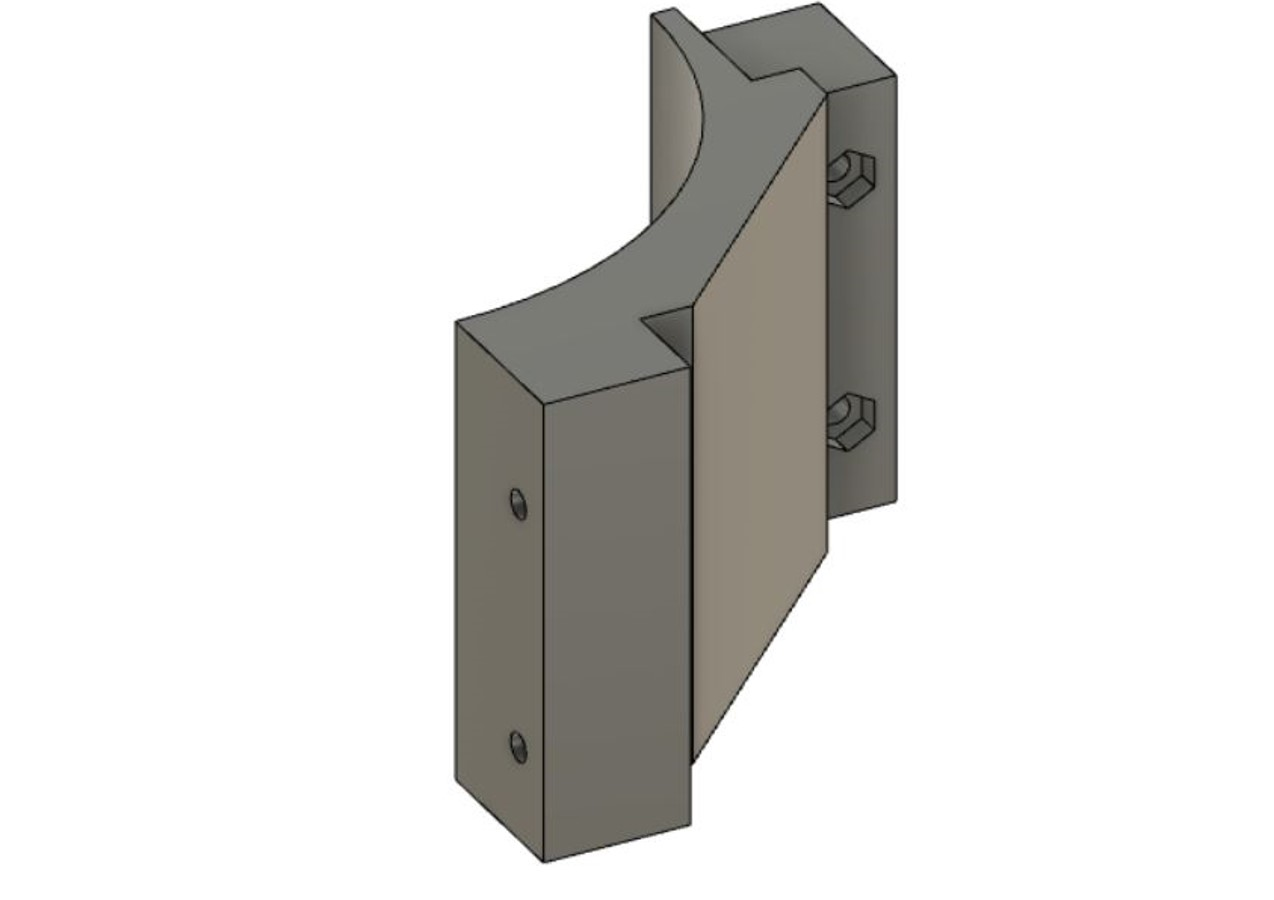
\includegraphics[width = 5.5cm]{coverpeice1}
			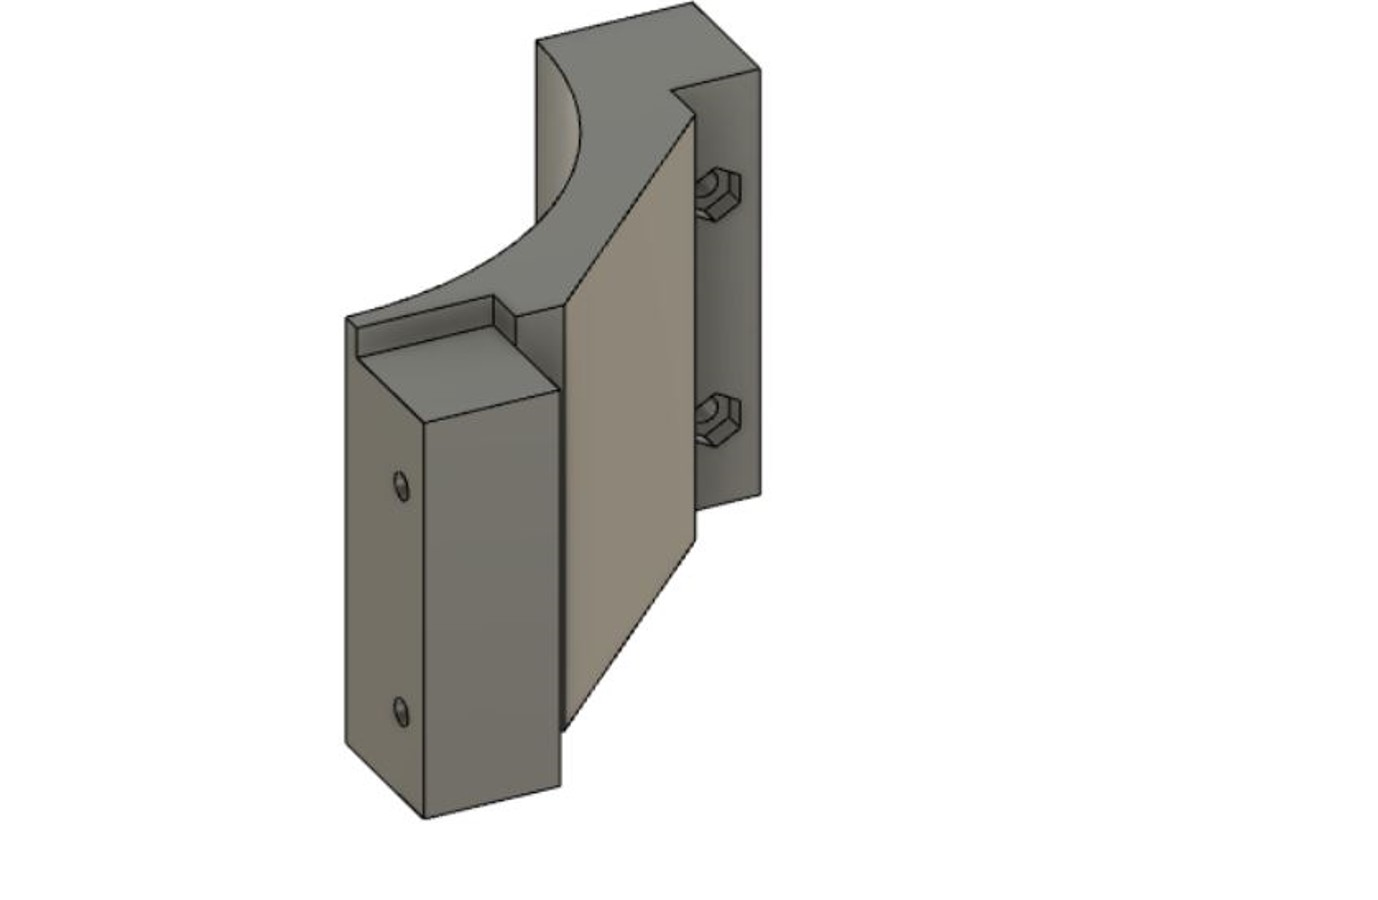
\includegraphics[width = 5.7cm]{coverpeice2}
	\end{center}
	\caption{Fusion360을 이용하여 설계한 경통 덮개조각들}
	\label{coverpeice}
\end{figure}

경통의 후드에서 바흐티노프마스크를 확실하게 제어하기 위해서는 바흐티노프마스크를 적용할 때와 적용하지 않을 때의 구분이 확실해야한다. 이를 확실하게 하기 위해서 바흐티노프마스크를 경첩을 이용하여 큰 각도로 제어하는 방법을 택하였으며, 이를 위해 덮개를 설계할 때 Fig. \ref{coverpeice}와 같이 경첩의 높이를 고려하여 제작하였다.

\subsection{바흐티노프마스크 제작}
천체망원경에 사용되는 대부분의 바흐티노프마스크의 도안은 직접 제작이 가능하며, 본 연구의 경우 astrojargon (http://astrojargon.net/MaskGenerator.aspx?AspxAutoDetectCookieSupport=1) 사이트에서 망원경의 사양 및 마스크의 사용 목적에 맞는 적절한 바흐티노프마스크의 도안을 제작하여 사용하였다.

덮개에서 사용되는 방식을 이용한 바흐티노프마스크의 경우 기존처럼 종이나 알루미늄에 프린트된 방식일 경우 덮개에 원하는 모양으로 씌워지지 않을 가능성이 있다. 때문에 주변환경에 영향을 적게 받으면서도 그 면이 평평하여 천체관측을 진행할 때에 영향이 없어야 한다. 


연구 초기에는 아크릴이 이러한 성질을 만족하면서도 쉽게 제작할 수 있으므로 아크릴에 레이저를 쐬여 바흐티노프마스크 모양을 씌우는 방법으로 테스트용 마스크를 제작해보았으나. 이러한 방식을 사용할 경우 Fig. \ref{bendmask}처럼 레이저로 인해 열을 받은 아크릴이 휘어 정밀한 초점 조절이 불가능해지는 경우가 발생하였으며, 아크릴의 두께로 인해 실제로 초점을 조절할 때에 걸리는 여러 가지 변수또한 무시할 수 없었다.

\bigskip
\begin{figure}[h]
	\begin{center}
		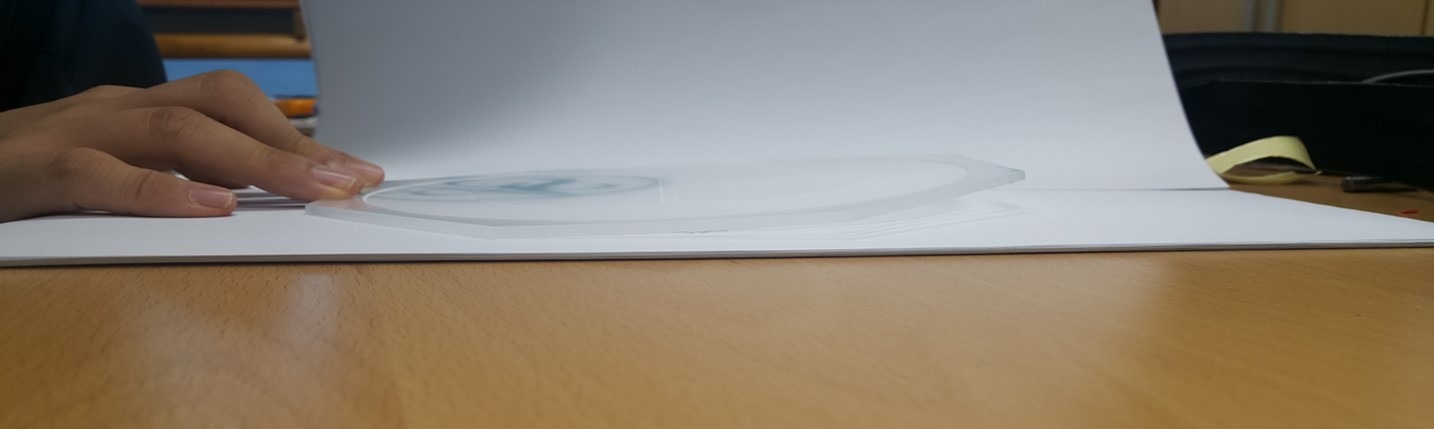
\includegraphics[width = 12 cm]{bendmask}
	\end{center}
	\caption{레이저에 의해 휘어진 아크릴 마스크}
	\label{bendmask}
\end{figure}


때문에 선택한 새로운 방법은 3d프린터를 이용하여 바흐티노프 마스크를 출력하는 것이다. 이러한 방법을 사용하면 얇으면서도 딱딱한 마스크를 사용할 수 있으므로 (보완해야합니다)~~~~~

\subsection{서보모터 제어}
 바흐티노프마스크를 제어하기 위해서 필요한 조건을 여러 가지가 있겠지만, 가장 중요한 조건 중 하나는 마스크를 사용하는 때와 그렇지 않을 때를 정확히 구분해야하며, 특히 마스크를 사용할 때에는 모든 상황에서 같은 환경을 제공할 수 있어야 한다. 본 연구에서는 경첩을 이용한 각도의 차이로 마스크를 제어하기 때문에 정확한 각도의 이동이 가장 중요하기 때문에 원하는 각도로 정확히 이동할 수 있는 서보모터를 사용하여 정확한 제어가 가능하도록 하였다.
 
\subsection{기존 모터포커서 보강}

앞서 소개했듯이 기존의 모터포커서인 GS-touch는 모터의 초점을 맞추기 위한 기능들에 집중이 되어있기 때문에, 실제로 천체관측 및 원격 천체관측에서는 사용하기 아쉬운 부분들이 많았다. 이에 기존 모터포커서를 보강하였으며, 기존 모터포커서에 비해서 원격 천체관측에 필요한 여러 가지 기능들을 탑재하였다. 본 연구에서 새로 보강한 부분은 다음과 같다.
\subsubsection{열선 제어}
열선또한 정확한 천체관측에 필요한 장비 중 하나이다. 관측을 진행할 때에 경통의 온도가 내려가면 렌즈에 이슬이 맺히게 되는데, 경통에 열선을 감아놓으면 경통의 온도에 따라서 열선을 제어하면 깨끗한 렌즈를 사용할 수 있으므로 뚜렷한 별 상을 얻을 수 있다.

\bigskip
\begin{figure}[h]
	\begin{center}
		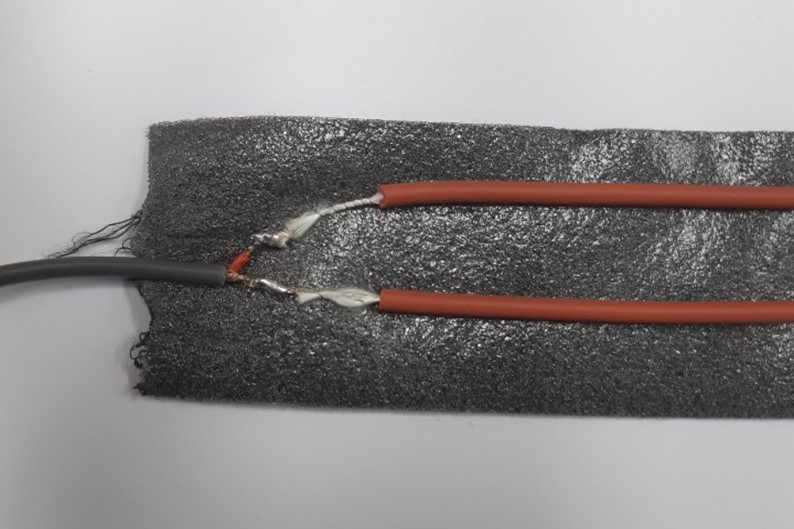
\includegraphics[width = 7 cm]{thermicline1}
	\end{center}
	\caption{제작한 열선의 접합부}
	\label{thermicline1}
\end{figure}

 먼저 Fig. \ref{thermicline1}처럼 끈끈한 면에 열선을 부착한 뒤에 Fig. \ref{thermiclin2e}처럼 전원선과 연결한다. 그리고 열선을 다시 덮어주게 되면 12V 전원을 통해 작동하는 열선을 제작할 수 있다. 열선을 실제로 사용할 시에는 그 편의성을 증대시키기 위해 열선의 끝부분을 벨크로로 연결할 수 있도록 만든다. 이렇게 제작한 열선은 경통에서 렌즈가 있는 부분을 찾아 둘러주면 벨크로로 끝을 고정시켜 쉽게 망원경에 부착시킬 수 있다.

 열선은 PWM(Puls Width Modulation)을 이용하여 세기를 조절할 수 있다. PWM은 디지털 신호의 밀도로 그 세기를 조절하는 방식으로, 아두이노 펌웨어 상에서는 다음과 같은 방법으로 구현할 수 있다.
 \bigskip
\begin{figure}[h]
	\begin{center}
		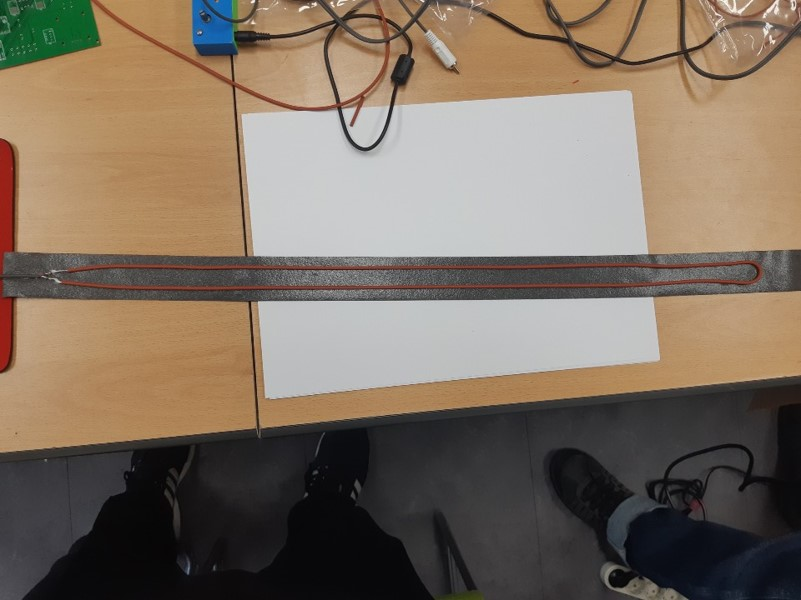
\includegraphics[width = 12 cm]{thermicline2}
	\end{center}
	\caption{열선의 내부 구조}
	\label{thermicline2}
\end{figure}

 대부분의 열선은 12V의 전압을 이용해 제어해야하기 때문에 아두이노의 출력 전원인 5V로는 신호만 제어하고, 스위칭 트랜지스터를 이용하여 12V의 전압을 PWM으로 제어하였다.

\subsubsection{EEPROM(Electrically Erasable Read-Only Memory)}

  mcu내에 원하는 값을 저장하는 방법은 여러 가지가 있다. 일반적으로 펌웨어가 실행되기 전에 변수를 선언하고, loop 문 속에 들어있는 여러 함수들을 통해 그 값을 바꾸는 방법을 사용하곤 한다. 하지만 원격 천체관측을 위한 펌웨어인 만큼, 그 전원을 계속 유지할 수 없기 때문에 다른 방법의 필요성을 느꼈다.
  
  EEPROM은 대표적인 롬(ROM - read only memory)의 한 종류로서, 전원을 차단해도 저장된 정보를 유지하는 비휘발성 메모리이다. eeprom은 address를 가지고 있어서 각각의 address 안에 지정된 bytes의 값을 저장할 수 있다. 본 연구에서 사용된 mcu인 Teensy 3.2는 0에서 1023까지의 address지를 가지고 있고 하나의 address에 2048byte, 즉 0부터 255까지의 수를 저장할 수 있다. 
 
  모터포커서의 step을 저장하기 위해서는 약 100000범위의 수를 저장할 필요가 있다. GS-touch는 약 -50000에서 50000까지의 수를 저장할 수 있기 때문에 256진법의 수를 활용하여 수를 저장하였다.
(eepread통해서 어떻게 저장하는지 설명)

 EEPcurrentPosition의 값을 loop문을 통해 현재 모터의 위치와 일치시키면 언제 전원이 꺼지더라도 EEPROM에 있는 값을 불러오면 편리하게 값을 저장할 수 있다.

%https://www.pjrc.com/teensy/td_libs_EEPROM.html
\begin{figure}[h]
	\begin{center}
		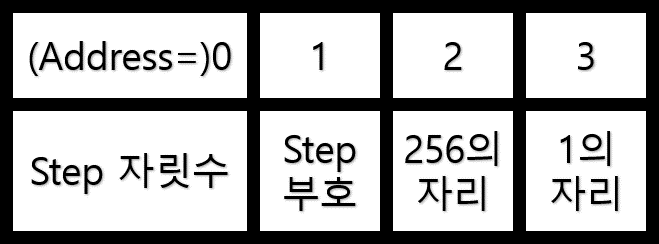
\includegraphics[width = 5 cm]{eeprom1}
	\end{center}
	\caption{EEPROM의 address별 사용 구조}
	\label{eeprom1}
\end{figure}

\subsubsection{서보모터 제어}

 서보모터는 일반적으로 사용하는 DC모터와 다르게 원하는 각도로 모터의 속도를 조절하여 이동시킬 수 있는 모터이다. 때문에 서보모터는 RC카의 방향제어, 로봇의 관절제어 등의 상황에서 자주 사용되며, 본 연구에서 사용되는 서보모터는 ‘ds lx3325mg 25kg’ 모델로, 서보모터이지만 360도 회전이 가능한 모델이다.
 
 \begin{figure}[h]
 	\begin{center}
 		\begin{tikzpicture}
 		\node[anchor=south west,inner sep=0] at (0,0) 
 		{
 			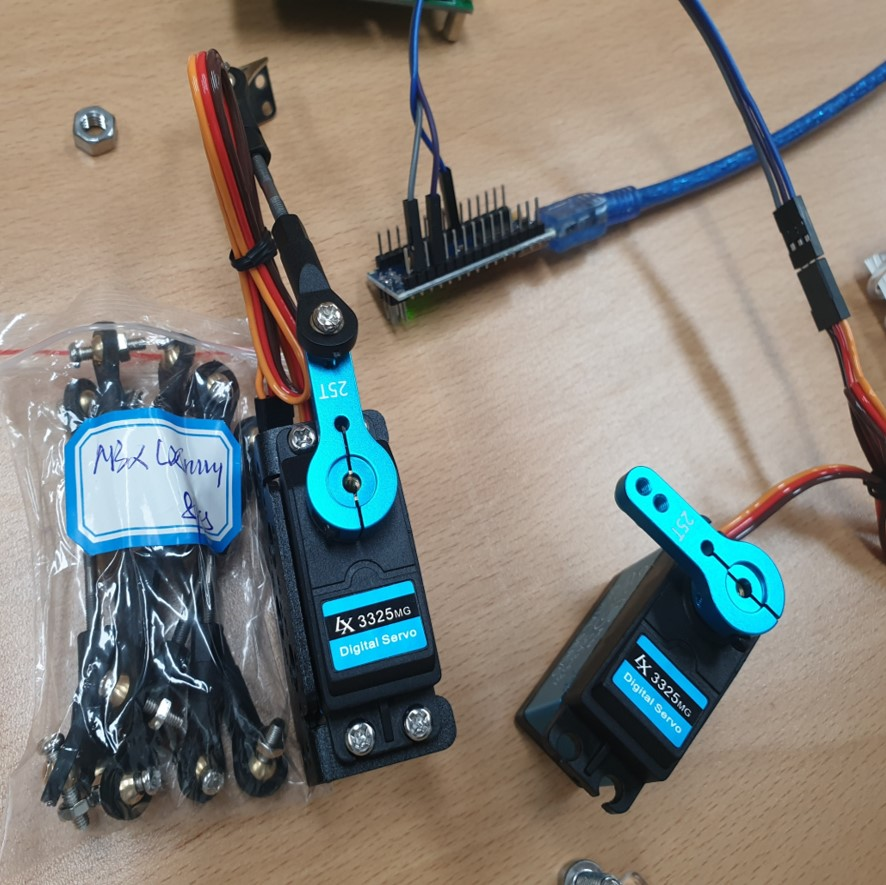
\includegraphics[width=6cm]{servo1}
 			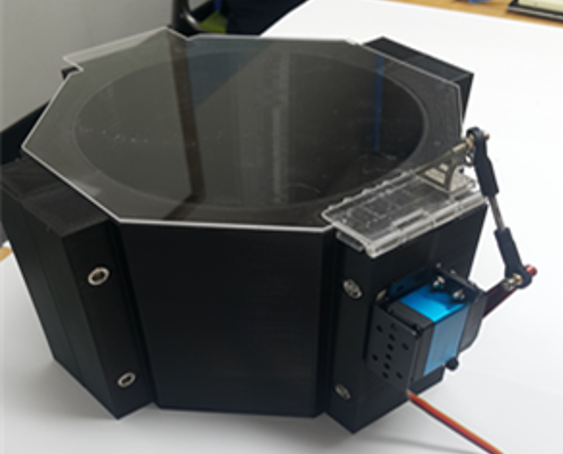
\includegraphics[width=6cm]{servo2} 
 		};
 		\draw (0.3, 5.7) node {(a)};
 		\draw (6.4, 5.7) node {(b)};
 		\end{tikzpicture}
 	\end{center}
 	\caption{(a) 사용한 서보모터인 ds lx3325mg 25kg와 (b) 이를 제작한 덮개에 장착한 모습.}
 	\label{motor}
 \end{figure}

 서보모터의 경우 구동을 위해 필요한 핀은 3가지이며, 일반적으로 주황색, 빨간색, 갈색의 핀으로 이루어져 있다. 주황색 핀은 모터를 제어할 수 있는 핀이며, 빨간색 핀과 갈색 핀은 각각 5v 전원과 GND에 연결하여 서보모터를 구동할 수 있다. 서보모터의 경우 Fig. \ref{motor}처럼 후드의 옆면에 부착시켜 일정한 각도로 제어할 수 있게끔 설계하였다.



\subsubsection{릴레이 스위치}

 릴레이 스위치는 전자석으로 이루어진 여러 스위치를 한번에 제어할 수 있도록 제작된 장비이다. 천체관측을 시작 및 종료할 때 가대, CCD, 카메라 등 한번에 여러 가지의 전원을 제어해야 하는데, 릴레이 스위치를 이용하면 한번에 제어할 수 있어 편리하다. 

 \begin{figure}[h]
	\begin{center}
		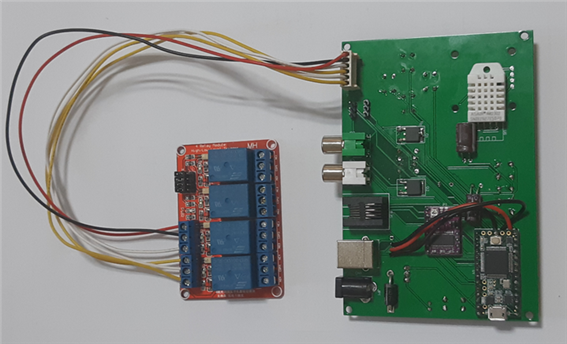
\includegraphics[width = 12cm]{relay}
	\end{center}
	\caption{실험에 사용된 릴레이스위치를 모터포커서에 연결시킨 모습}
	\label{relay}
\end{figure}

 Fig. \ref{relay}와 같이 각각의 스위치를 선으로 연결시켜 mcu의 각 핀에 연결시켜 작동시킬 수 있으며, 함수로 지정하여 이들을 한번에 제어할 수 있도록 하였다.
 
\newpage
\section{연구 결과}

\subsection{천체망원경의 덮개}

 \begin{figure}[h]
	\begin{center}
		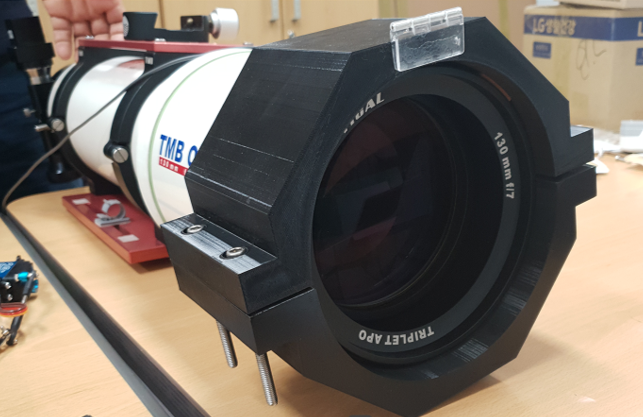
\includegraphics[width = 12cm]{cover}
	\end{center}
	\caption{제작한 덮개를 천체망원경에 씌운 모습}
	\label{cover}
\end{figure}

\newpage
\subsection{개선된 모터포커서}


 \begin{figure}[h]
	\begin{center}
		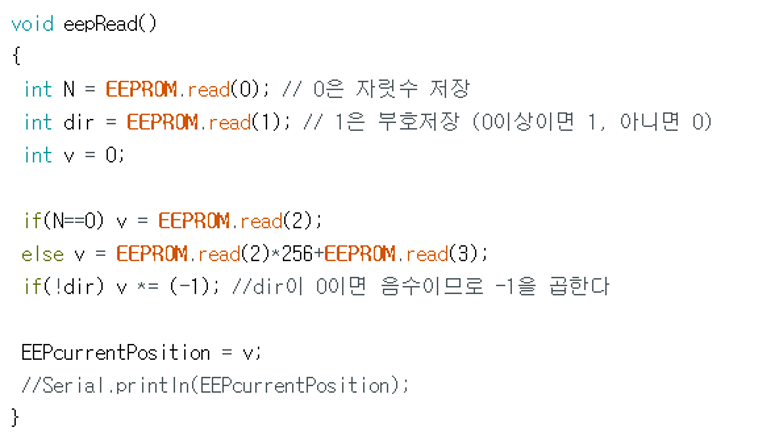
\includegraphics[width = 12cm]{eepread}
	\end{center}
	\caption{EEPROM에서 정보를 읽어오는 과정}
	\label{eepread}
\end{figure}

 \begin{figure}[h]
	\begin{center}
		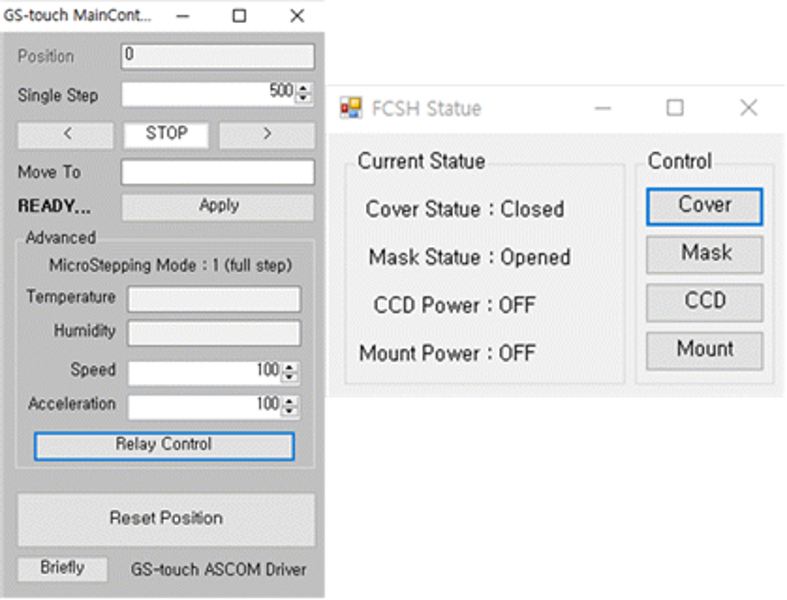
\includegraphics[width = 12cm]{maincontrol}
	\end{center}
	\caption{개선된 모터포커서 드라이버의 GUI 모습}
	\label{maincontrol}
\end{figure}



\newpage
\section{결론 및 제언}
\subsection{결론}
  본 연구는 원격 천체관측을 편리하게 하기 위해 필요한 여러 시스템들을 기존에 개발된 모터포커서를 이용하여 원격 천체관측에 도움이 되는 것을 목적으로 하였으며, 이를 위한 바흐티노프 마스크 제어용 망원경 덮개 및 시험 동작을 시행하였다. 본 제어시스템을 개발하기 위해 사용한 틀은 EasyEDA, Fusion 360, Arduino IDE, Visual Studio 2017, ASCOM flatform 등을 포함하여 이들의 효율적인 사용을 위한 여러 라이브러리가 사용되었으며, 이들의 원리를 적절히 응용하여 제작하였다. 

본 연구의 결과물을 요약하면 다음과 같다.

 첫째, 3D프린터와 망원경의 경통 구조를 적절히 활용하여 바흐티노프 마스크의 제어가 가능한 덮개를 개발하였다. 덮개의 크기 때문에 일반적인 3D프린터로 출력하기 힘들어 네 부분으로 나누어 출력하였으며, 경첩을 이용하여 마스크를 제어하기 때문에 경첩이 들어갈 부분을 만들어주었다. 경첩은 같은 방향에 부착된 서보모터를 이용하여 제어되며, 서보모터는 항상 같은 각도로 움직일 수 있기 때문에 경첩과 마스크를 동작시킬때의 안정성이 매우 뛰어나다.
 
 둘째, 천체망원경의 원격 제어 및 덮개의 원활한 동작을 위해 모터포커서를 개선하였다. 개선한 부분은 크게 네 가지로. 열선의 제어, EEPROM 적용, 덮개의 제어를 위한 서보모터 제어, 전원 동작의 편리함을 더하는 릴레이스위치의 제어로 나놀 수 있다. 또한 새로 생긴 기능들을 적절히 활용할 수 있도록 포커서 컨트롤 소프트웨어의 기능들 또한 개선하였다.

 현재 망원경을 사용하기 위해서는 미리 덮개를 열고 있어야 한다. 하지만 덮개를 열고 있는 상태에서 먼지가 경통의 속으로 들어가게 되는 단점이 존재하게 되어 이는 원격 천체망원경의 제어에 큰 어려움이 된다. 하지만 이번 연구를 통해서 덮개를 미리 열고 있어야 하는 단점을 없애 먼지가 최대한 안 들어오도록 할 수 있게 되었고, 덮개로 바흐티노프마스크를 제어할 수 있게 되어 포커서 컨트롤러를 만들어 초점을 맞출 때 v-curve를 그릴 필요 없이 초점을 맞출 수 있게 되었으며, 열선을 설치하여 렌즈에 이슬이 맺히는 것을 방지하여 좀 더 좋은 별 상을 얻을 수 있게 될 것으로 예상된다.

\subsection{제언}

 \newpage
\subsection{Figures}
논문에 들어가는 그림은 크게 사진과 그래프로 나눌 수 있다. 먼저 사진파일(확장자 jpg, png)을 넣는 방법은 다음과 같다.
\begin{center}
\fbox{\parbox{0.9\textwidth}{
{\textbackslash}begin\{figure\}[t]\\
{\textbackslash}begin\{center\}\\
{\textbackslash}includegraphics[width=6cm]\{Figure File\}\\
{\textbackslash}caption\{This is caption\}\\
{\textbackslash}label\{Figure label\}\\
{\textbackslash}end\{center\}\\
{\textbackslash}end\{figure\}
}}\end{center}
{\textbackslash}begin\{figure\} 옆의 [t]라는 옵션은 그림을 페이지의 맨 위에 넣는다는 것이다. 옵션의 종류는 t, b, h, p가 있다. 각각의 의미는, t : 그림을 페이지 맨 위에 위치, b : 그림을 페이지 맨 아래에 위치, h : 그림을 본문에 작성한 위치에 넣기. 단 충분한 공간이 없는 경우에는 다음 페이지에 들어감, p : 한 페이지에 그림만 등장함. 논문에 등장하는 그림들은 되도록 페이지 위에 위치할 수 있도록 하자. 즉 [t] 옵션을 설정한다. 단, section title이 맨 위에 위치하는 경우에는 [b] 옵션을 사용하여 그림을 페이지 바닥에 위치시킨다.

includegraphics다음의 [ ] 안에는 크기를 지정할 수 있는 옵션을 넣어주고 \{ \} 안에는 파일이름(확장자 포함)을 넣어준다. 이때 그림 파일은 \LaTeX\ 파일과 같은 폴더에 들어 있어야 한다. 다음의 caption에는 그림 설명을 넣어준다. 마지막으로 label에는 수식에서와 마찬가지로 이 그림의 라벨을 지정하여 본문 속에서 ref 명령어를 사용하여 그림을 언급하기 편하도록 한다.

이번에는 그래프를 넣는 방법을 알아보자. 그래프는 사진과 약간 차이가 있는데 그것은---엑셀 등 그래프 작성 툴에서 그래프를 그린 후 그래프를 그림파일로 저장할 때, 확장자 pdf, eps 등 postscript 계열의 벡터 이미지로 저장을 해야 한다는 것이다. 그 외에는 사진 이미지 삽입과 동일하다. 그림 \ref{Fig01}은 엑셀에서 작성한 그래프를 pdf로 저장한 것 (왼쪽)과 png로 저장한 것 (오른쪽)을 비교하기 위한 예이다. 컴파일 후 생성된 논문 pdf파일을 확대해보면 그 차이를 알 수 있다.

\begin{figure}[t]
\begin{center}
\includegraphics[width=6cm]{Fig01a.pdf}
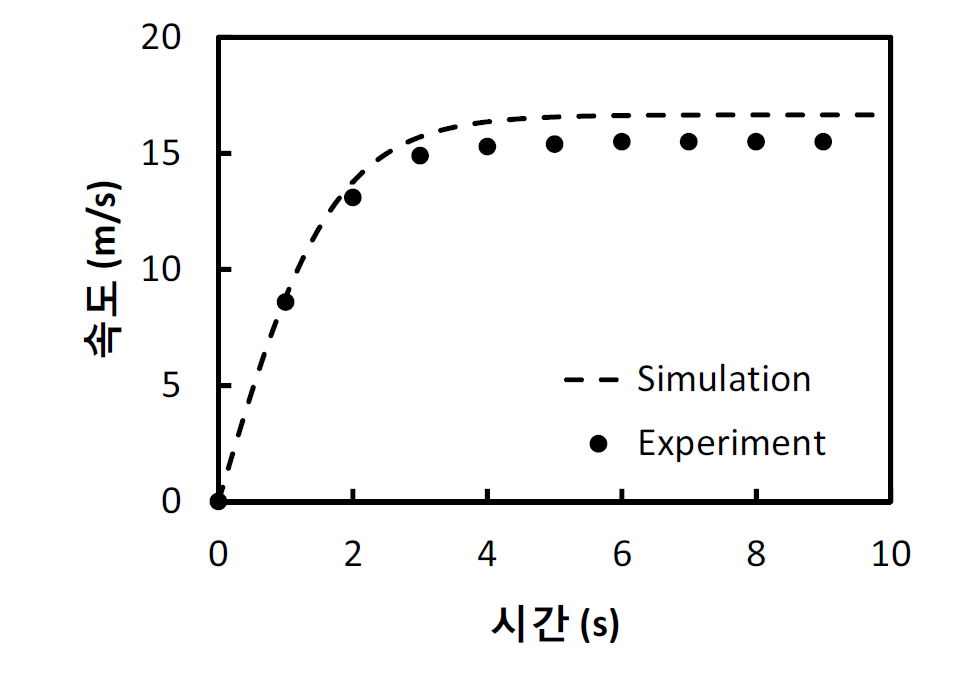
\includegraphics[width=6cm]{Fig01b.png}
\caption{The example to show the difference between a vector image (left) and a dot image (right).} \label{Fig01}
\end{center}
\end{figure}

Figure \ref{Fig01}처럼 figure 명령어 안에 여러 개의 그림 객체를 포함시키는 경우 캡션에서는 각 객체마다 설명을 작성해야 한다. 그림이 좌우 두 개로 구성된 경우 괄호 안에 왼쪽(또는 left), 오른쪽 (또는 right)와 같이 표시하면 되지만 세 개 이상의 그림을 묶어줄 때는 (a), (b), (c), ...처럼 하위 라벨을 붙여준다. 하위 라벨 표기는 크게 그림 파일을 제작할 때 하위 라벨을 포함시키는 방법과, \TeX에서 작성하는 방법으로 나눌 수 있다. 먼저 그림 파일 제작 때 하위 라벨 작성을 포함시키는 방법은 앞에서 설명한 그림 삽입 방법과 동일하며 \TeX\ 파일 작성에서의 편리함이 있지만, 그림 교체, 순서 변경, 크기 조절 등이 있을 때마다 그림 파일을 다시 제작해야 하는 단점이 있다. 반면 \TeX에서 하위 라벨을 작성하는 경우에는 이런 단점은 사라진다. \TeX에서 하위 라벨을 입력하는 방법은 다양하다. {\textbackslash}begin\{figure\} 명령어 이후 i) subfigure 명령어를 사용하는 방법, ii) minipage를 사용하는 방법, iii) tabular를 사용하는 방법 등. 여기서는 overpic 패키지의 overpic 명령어를 사용하는 방법을 소개한다. 다음과 같이 입력하고 컴파일을 하면 Figure \ref{Fig02}와 같은 그림 세트를 얻는다. 여기서 {\textbackslash}put 명령어 다음에 사용된 숫자 (25,60)은 왼쪽으로부터 그림 넓이의 25\%, 아래로부터 그림 높이의 60\% 되는 위치에 텍스트를 입력한다는 의미이다.

\begin{center}
\fbox{\parbox{0.9\textwidth}{
{\textbackslash}usepackage[percent]\{overpic\}\\
\par
{\textbackslash}begin\{document\}\\
\\
{\textbackslash}begin\{figure\}[t]\\
{\textbackslash}begin\{center\}\\
{\textbackslash}begin\{overpic\}[width=5.6cm]\{Fig02a.pdf\}{\textbackslash}put(25,60)\{(a)\}{\textbackslash}end\{overpic\}\\
{\textbackslash}begin\{overpic\}[width=5.6cm]\{Fig02b.pdf\}{\textbackslash}put(25,60)\{(b)\}{\textbackslash}end\{overpic\}{\textbackslash}{\textbackslash}\\
{\textbackslash}begin\{overpic\}[width=5.6cm]\{Fig02c.pdf\}{\textbackslash}put(25,60)\{(c)\}{\textbackslash}end\{overpic\}\\
{\textbackslash}begin\{overpic\}[width=5.6cm]\{Fig02d.pdf\}{\textbackslash}put(25,60)\{(d)\}{\textbackslash}end\{overpic\}\\
{\textbackslash}end\{center\}\\
{\textbackslash}caption\{Cation here\}\\
{\textbackslash}label\{Fig02\}\\
{\textbackslash}end\{figure\}
}}\end{center}

\begin{figure}[h]
\begin{center}
\begin{overpic}[width=5.6cm]{Fig01a.pdf}\put(25,60){(a)}\end{overpic}
\begin{overpic}[width=5.6cm]{Fig01a.pdf}\put(25,60){(b)}\end{overpic}\\
\begin{overpic}[width=5.6cm]{Fig01a.pdf}\put(25,60){(c)}\end{overpic}
\begin{overpic}[width=5.6cm]{Fig01a.pdf}\put(25,60){(d)}\end{overpic}
\end{center}
\caption{Total title of this figure. (a) subfigure 1 explanation (b) subfigure 2 explanation (c) subfigure 3 explanation (d) subfigure 4 explanation}\label{Fig02}
\end{figure}

논문에 그림을 넣을 때 주의사항은 다음과 같다.
\begin{itemize}
\item{논문에 반드시 필요한 그림인가.}\\[-34pt]
\item{남들이 이해하는데 있어서 가장 알맞은 형태로 표현되었는가.}\\[-34pt]
\item{캡션과 본문에서의 설명은 충분한가.}
\end{itemize}
대부분의 연구자들이 다른 사람이 저술한 논문을 읽을 때 가장 먼저 보는 것이 잘 시각화 된 그림이다. 따라서 그림은 논문 내용의 핵심을 담고 있어야 하며, 간결하고 이해하기 쉬워야 한다. 종종 그림을 잘 취합하거나 더 좋은 형태의 데이터로 승화시키지 못하고, 여러 쪽에 걸쳐 그림만 남발하는 논문을 작성하는 학생들도 있다. 원래는 독자가 그림을 먼저 보고 호기심이 자극되어 논문의 본문을 읽도록 해야하는데, 그림이 지나치게 많은 논문은 그림 읽기 단계부터 피로감을 발생시켜 독자에게 불편함을 느끼게 한다. 원칙이 있는 건 아니지만, 글과 그림의 페이지 점유 정도를 비교할 때 글이 차지하는 비중을 높게 하도록 한다. 본인이 작성한 논문에서 그림의 양이 너무 많다면 그림의 양을 줄이고 글의 양을 늘려보자. 만약 글로 설명할 수 있는 분량이 충분치 않다면 아마도 그 그림은 논문에서 빠져도 상관없는 그림일 것이다.

\subsection{Tables}

\LaTeX에서 표를 넣는 방법은 i)엑셀 등 외부 프로그램에서 작성된 표를 pdf 그림파일로 변환하여 그림처럼 includegraphics 명령어로 넣는 방법 (물론 이 경우 {\textbackslash}begin\{figure\} 대신 {\textbackslash}begin\{table\}를 사용해야 함), ii)\LaTeX에서 표를 직접 제작하는 방법의 두 가지가 있다. \LaTeX에서는 명령어에 의해 표의 구획과 정렬, 선의 종류를 표현하므로 초보자에게는 다소 어려운 작업이 될 수 있다. 아마도 \LaTeX를 사용함에 있어서 가장 불편한 점은 표 제작 작업일 것이다. 다행히 인터넷에 `latex', `table' 등의 조합으로 검색하면 마우스로 제작한 표를 \LaTeX로 변환해주는 웹사이트들을 찾을 수 있다.

다음은 간단한 표의 예이다. 다음과 같이 입력을 하고 컴파일을 하면,
\begin{center}
\fbox{\parbox{0.9\textwidth}{
{\textbackslash}begin\{table\}[t]\\
{\textbackslash}caption\{Physical parameters.\}\\
{\textbackslash}label\{table01\}\\
{\textbackslash}begin\{center\}\\
{\textbackslash}begin\{tabular\}\{c $|$ c $|$ c\}\\
{\textbackslash}hline\\
 \& symbol \& value {\textbackslash}{\textbackslash} {\textbackslash}hline \\
Earth's mass \& \$M\_E\$ \& \$6.0{\textbackslash}times 10$\hat{\ }$\{24\} \{{\textbackslash}rm kg\}\$ {\textbackslash}{\textbackslash}\\
Earth's radius \& \$R\_E\$ \& \$6.4{\textbackslash}times 10$\hat{\ }$6 \{{\textbackslash}rm m\}\$ {\textbackslash}{\textbackslash}\\
Gravitational constant \& \$G\$ \& \$6.67{\textbackslash}times 10$\hat{\ }$\{-11\} \{{\textbackslash}rm N m$\hat{\ }$2 /kg$\hat{\ }$2\}\$ {\textbackslash}{\textbackslash} \\
{\textbackslash}hline\\
{\textbackslash}end\{tabular\}\\
{\textbackslash}end\{center\}\\
{\textbackslash}end\{table\}
}}\end{center}
Table \ref{table01}과 같은 표를 얻게 된다.
\begin{table}[t]
\caption{Physical parameters.} \label{table01}
\begin{center}
\begin{tabular}{c|c|c}
\hline
 & symbol & value \\ \hline
Earth's mass & $M_E$ & $6.0\times 10^{24} {\rm kg}$ \\
Earth's radius & $R_E$ & $6.4\times 10^6 {\rm m}$ \\
Gravitational constant & $G$ & $6.67\times 10^{-11} {\rm N m^2 /kg^2}$ \\ \hline
\end{tabular}
\end{center}
\end{table}


%-----------------------------------------------------
% Conclusion
%-----------------------------------------------------

\section{결론}
글이라는 것은 개인의 개성이 담겨 있기 때문에 모든 사람들이 동일한 방식으로 표현하는 것은 아니다. 그러나 예로부터 개인의 연구 내용을 글로써 타인에게 전달할 때, 효율적인 방법이라고 공감대를 형성하며 다듬어져 온 것이 지금의 논문 형태이다. 그러므로 처음 논문을 작성하는 학생들은 이 문서에서 지시하는 논문 작성 방식을 따르는 것을 권한다. 하지만 여기서는 다양한 논문들에 대해 일일이 사례를 들어 올바른 논문 작성법을 설명하기에는 한계가 있기에 간략하게만 소개를 했다. 여기서 설명되지 않은 부분들은 다른 사람들의 논문을 참고하자. 이미 서론을 작성하면서 많은 선행 연구 논문들을 읽어 봤을 것이다. 그 논문들에서는 데이터를 어떤 방식으로 표현하는지, 서론은 어떤 흐름으로 구성하는지 등을 살펴보자. 논문을 잘 쓰는 비결의 첫 번째는 논문을 많이 읽어 보는 것이다.


%-----------------------------------------------------
% Appendix  (Appendix가 없는 경우 이 파트 전체를 제거하시오)
%-----------------------------------------------------
\clearpage  %%% Appendix를 새 페이지에서 시작
\appendix
\renewcommand{\thesection}{\Alph{section}} %%% TOC에 appendix numbering 재설정
\titleformat{\section}[hang] {\normalfont\LARGE\bfseries}{\Alph{section}.}{1em}{} %%% Appendix section title의 재설정
\renewcommand{\theequation}{\thesection.\arabic{equation}} %%% Appendix equation numbering 의 재설정
\renewcommand{\thefigure}{\thesection-\arabic{figure}} %%% Appendix figure numbering 의 재설정
\renewcommand{\thetable}{\thesection-\arabic{table}} %%% Appendix table numbering 의 재설정
\setcounter{equation}{0} %%% Appendix equation starting number의 초기화
\setcounter{figure}{0} %%% Appendix figure starting number의 초기화
\setcounter{table}{0} %%% Appendix table starting number의 초기화

\section{Appendix title}
논문의 구조 상 본문에 넣지는 못했지만 논문에 수록하고 싶은 부록(appendix)이 있다면 여기에 작성한다. Appendix는 반드시 있어야 하는 건 아니다. 만약 본문에서 연구 내용을 충분히 작성했다면 이 Appendix 파트 전체를 제거한다. 되도록 Appendix 작성을 자제하고 본문에서 설명할 수 있도록 한다.


%-----------------------------------------------------
%   References
%-----------------------------------------------------
\clearpage
\begin{thebibliography}{99}\begin{onehalfspace}

\bibitem{Mok10}C. Mok, C.-M. Ryu, P. H. Yoon, and A. T. Y. Lui, ``Obliquely propagating electromagnetic drift ion cyclotron instability'', J. Geophys. Res., {\bf 115}, A04218 (2010).
\bibitem{Schindler74} K. Schindler, ``A theory of the substorm mechanism'', J. Geophys. Res., {\bf 79}, 2803 (1974).
\bibitem{Sitnov97} M. I. Stinov, H. V. Malova, and A. T. Y. Lui, ``Quasi-neutral sheet tearing instability induced by electron preferential acceleration from stochasticity'', J. Geophys. Res., {\bf 102}, 163 (1997).
\bibitem{Zelenyi08} L. Zelenyi, A. Artemiev, H. Malova, and V. Popov, ``Marginal stability of thin current sheets in the Earth's magnetotail'', J. Atmos. Sol. Terr. Phys., {\bf 70}, 325 (2008).
\bibitem{Cheng98} C. Z. Cheng and A. T. Y. Lui, ``Kinetic ballooning instability for substorm onset and current disruption observed by AMPTE/CCE'', Geophys. Res. Lett., {\bf 25}, 4091 (1998).
\bibitem{Bhattacharjee98} A. Bhattacharjee, Z. W. Ma, and X. Wang, ``Dynamics of thin current sheets and their disruption by ballooning instabilities: A mechanism for magnetospheric substorms'', Phys. Plasmas, {\bf 5}, 2001 (1998).
\bibitem{Dobias04} P. Dobias, I. O. Voronkov, and J. C. Samson, ``On linear plasma instabilities during the substorm expansive phase onset'', Phys. Plasmas, {\bf 11}, 2046 (2004).
\bibitem{Zhu03} P. Zhu, A. Bhattacharjee, and Z. W. Ma, ``Hall magnetohydrodynamic ballooning instability in the magnetotail'', Phys. Plasmas, {\bf 10}, 249 (2003).
\bibitem{Saito08} M. H. Saito, {\it et. al.}, ``Ballooning mode waves prior to substorm-associated dipolarizations: Geotail observations'', Geophys. Res. Lett., {\bf 35}, L07103 (2008).
\bibitem{Friedrich01} E. Friedrich, J. C. Samson, and I. Voronkov, ``Ground-based observations and plasma instabilities in auroral substroms'', Phys. Plasmas, {\bf 8}, 1104 (2001).
\bibitem{Shinohara98} I. Shinohara, {\it et. al.}, ``Low-frequency electromagnetic turbulence observed near the substorm onset site'', J. Geophys. Res., {\bf 103}, 20,365 (1998).
\bibitem{Yoon02} P. H. Yoon, A. T. Y. Lui, and M. I. Sitnov, ``Generalized lower-hybrid drift instabilities in current-sheet equilibrium'', Phys. Plasmas, {\bf 9}, 1526 (2002).
\bibitem{Mok06}C. Mok, C.-M. Ryu, P. H. Yoon, and A. T. Y. Lui, ``Global two-fluid stability of bifurcated current sheets'', J. Geophys. Res., {\bf 111}, A03203 (2006).
\bibitem{Rostoker84} G. Rostoker and J. C. Samson, ``Can substorm expansive phase effects and low frequency Pc magnetic pulsations be attributed to the same source mechanism?'', Geophys. Res. Lett., {\bf 11}, 271 (1984).
\bibitem{Dovias06} P. Dovias, J. A. Wanliss, and J. C. Samson, ``Nonlinear stability of the near-Earth plasma sheet during substorms: 9 February 1995 event'', Can. J. Phys., {\bf 84}, 1029 (2006).
\bibitem{Yoon93} P. H. Yoon and A. T. Y. Lui, ``Nonlinear analysis of generalized cross-field current instability'', Phys. Fluids B, {\bf 5}, 836 (1993).
\bibitem{Sadovskii01} A. M. Sadovskii and A. A. Galeev, ``Quasilinear theory of the ion Weibel instability in the Earth's magnetospheric tail'', Plasma Phys. Rep., {\bf 27}, 490 (2001).
\bibitem{Yoon06} P. H. Yoon and A. T. Y. Lui, ``Quasi-linear theory of anomalous resistivity'', J. Geophys. Res., {\bf 111}, A02203 (2006).

\end{onehalfspace}\end{thebibliography}

%-----------------------------------------------------
%   Summary (영어로 작성한 학생은 이 부분 전체를 제거한다.)
%-----------------------------------------------------
\begin{summary}
\addcontentsline{toc}{section}{Summary}  %%% TOC에 표시
한글로 졸업논문을 작성한 학생은 반드시 5페이지 내외의 영어 요약문을 작성해야 합니다. 영문으로 작성하는 학생은 이 부분을 작성하지 않아도 됩니다.
\end{summary}

%-----------------------------------------------------
%   감사의 글
%-----------------------------------------------------
\begin{acknowledgements}
\addcontentsline{toc}{section}{감사의 글}  %%% TOC에 표시
정말 감사합니다.
\end{acknowledgements}

%-----------------------------------------------------
%   연구활동
%-----------------------------------------------------
\begin{researches}
\addcontentsline{toc}{section}{연구활동}  %%% TOC에 표시
\begin{itemize}
\item{2017학년도 교내 R\&E 발표대회에서 장려상 수상}
\item{2018학년도 교내 R\&E 발표대회에서 장려상 수상}
\item{2019년 노벨 물리학상 수상}
\end{itemize}
\end{researches}


\end{document} 